% !TEX root = ../main.tex

\section{The Rust Programming Language} % (fold)
\label{sub:the_rust_programming_language}

Rust \cite{web:rust_lang} is a new open source systems programming language developed by the Mozilla Foundation \cite{web:mozilla_foundation}.
It is designed to support concurrency and parallelism and take full utilization of the underlying hardware.
Rust makes strong guarantees about isolation and memory safety, while still focusing on performance.

Rust is a strongly and statically typed, multi-paradigm programming language.
The language borrows many traits and features from other, already existing languages.
The following subsections discusses some of the more prominent language features, that all work together in order to achieves Rust's main goals; mainly full memory safety without sacrificing performance.
\todo{I've just been throwing out ideas and statements that are probably not very true.}

\subsection{Language Features}
\label{ssub:rust:features}

This section describes a few key language features of Rust that are not present in the procedural paradigm usually found in embedded programming.
The language is multiparadigm and therefor offeres a wider range of language constructs.

\subsubsection{Sum types - Enum}

The \textbf{enum} type of Rust is a powerful construct.
The type is based on sum types and can hold tagged data in addition to named values as enumerated types as found in C.
A canonical example of a Sum type is the representation of a linked list in \autoref{lst:rust:list}.

\begin{listing}[H]
  \begin{minted}{rust}
    enum List<T> {
      Cons(T, Box<List>),
      Nil,
    }
  \end{minted}
  \caption{Definition of Linked List}
  \label{lst:rust:list}
\end{listing}

Each list item is either a value and a pointer to the next item, as the \textbf{Cons}, or a termination value as \textbf{Nil}.

\subsubsection{Case Study - Option}

\begin{listing}[H]
  \begin{minted}{rust}
    pub enum Option<T> {
      Some(T),
      None,
    }
  \end{minted}
  \caption{Definition of Option}
  \label{lst:rust:option}
\end{listing}

\subsubsection{Pattern Matching and Destruction}

Pattern matching is a language construct that resembles the switch statement of "C-type" languages, but it is more powerful.
In addition to choose the matching tag/value, as a conventional switch does, the matching construct is able to destruct the matching value.
An example using the pattern matching on a Option type is given in Listing \ref{lst:rust:match}.

\begin{listing}[H]
  \begin{minted}{rust}
    let option: Option<u32> = Some(42);

    match option {
      Some(number) => println!("{}", number),
      None => (),
    }
  \end{minted}
  \caption{Matching an Option}
  \label{lst:rust:match}
\end{listing}

In Listing \ref{lst:rust:match} the Option \texttt{Some(42)} is checked against the patterns in the match expression.
As the first pattern matches the value, the number \texttt{42} is bound to the variable number and the \texttt{println} function is executed.

\subsubsection{Traits}

A Trait defines behavior for an object that implements the Trait.
Traits are used to facilitate code reuse and polymorphism.

One integral trait in the Rust programming language is the Iterator trait defined in Listing \ref{lst:rust:iterator}.

\begin{listing}[H]
  \begin{minted}{rust}
    pub trait Iterator {
      type Item;
      fn next(&mut self) -> Option<Self::Item>;
      fn size_hint(&self) -> (usize, Option<usize) { (0, None) }
      // ...
    }
  \end{minted}
  \caption{Definition of Iterator trait}
  \label{lst:rust:iterator}
\end{listing}

Implementing the Iterator trait for the List type in Listing \ref{lst:rust:list-iter} involves the discussed features enums, pattern matching and traits.

\begin{listing}[H]
  \begin{minted}{rust}
    impl<T: Clone> Iterator for List<T> {
      type Item = T;

      fn next(&mut self) -> Option<T> {
        match self.clone() {
          Cons(val, next) => {
            *self = *next;
            Some(val)
          },
          Nil => None
        }
      }
    }
  \end{minted}
  \caption{Implementing the Iterator trait for the List type}
  \label{lst:rust:list-iter}
\end{listing}


\subsubsection{Loops}

Rust provides the two known loop constructs \textbf{for} and \textbf{while}, in addition to \textbf{loop} for infinite loops.
The \textbf{for} loop is not the conventional \textit{for (initialize; condition; increment)}, it operates on iterators.
To understand the functionality we look the approximate desugaring of the for loop into a loop and a match expression in Listing \ref{lst:rust:for}


\begin{minipage}[b]{0.5\linewidth}
  \begin{listing}[H]
  \begin{minted}{rust}

    let values = vec![1, 2, 3];
    for x in 0..10 {
      println!("{}", x);
    }

  \end{minted}
  \caption{Desugaring for loop}
  \label{lst:rust:for}
  \end{listing}
  \end{minipage}

\begin{minipage}[b]{0.5\linewidth}
  \begin{listing}[H]
    \begin{minted}{rust}

      let mut it = values.into_iter();
      loop {
        match it.next() {
          Some(x) => println!("{}", x),
          None => break,
        }
      }

    \end{minted}

    \caption{Desugaring for loop}
    \label{lst:rust:desugared-for}
  \end{listing}
\end{minipage}

\subsubsection{Case Study - Result}

The Result type is an integral type in the Rust library and in Rust code in general.
The type is the base type for error handling.

\begin{listing}[H]
  \begin{minted}{rust}
    #[must_use]
    pub enum Result<T, E> {
      Ok(T),
      Err(E),
    }
\end{minted}
\caption{Definition of Result}
\label{lst:rust:result}
\end{listing}

\subsection{Zero-cost Abstractions}
\label{chap:zero_cost_abstractions}

Abstractions, in the form of references and pointers to objects or structures and how they are
structured on the heap, is a common source of overhead in programming languages.
\autoref{fig:java_abstractions} \todo{Update with nicer figure} shows how Java lays out a vector of
strings in memory.
A reference to the heap-allocated vector is placed on the stack, and the vector itself stores internal references to different strings that is placed elsewhere on the heap.
Thus, if the programmer wants to access the first character of a string, two objects have to be found and dereferenced on the heap in order to read the value;

\begin{enumerate}
  \item the vector must be dereferenced so that a reference to the string can be returned, and
  \item the string must be dereferenced so that character can be read.
\end{enumerate}

If the nesting of objects is deep it can result in many unnecessary heap-lookups in order to get the desired data.

\begin{figure}[tb]
  \begin{center}
    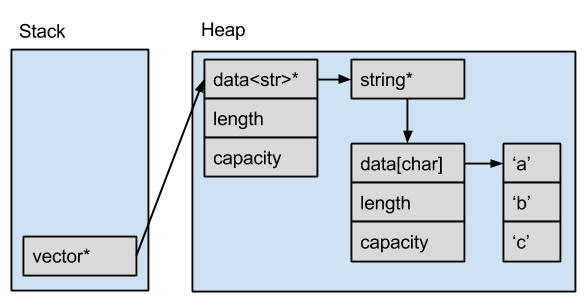
\includegraphics[scale=0.5]{figures/java_abstractions}
  \end{center}
  \caption{Abstractions of a Vector of Strings in Java.}
  \label{fig:java_abstractions}
\end{figure}

Rust introduces the same zero-cost abstractions that are featured in C and C++, among others.
This is both important for performance, and generally in order to have a deterministic and a common understanding of how the structures are laid out in the memory when working with embedded devices.
\todocite{This is a bogus sentence. Also, need to cite zero-cost abstraction articles}
\autoref{fig:cpp_abstractions} shows how C++ places the structures in memory.
The main difference is that the structure data itself is placed on the stack and inside the vector, instead of the references to the structures, yet keeping the same level of abstraction.
In Rust's case, all structures is allocated directly on the stack if it is not shared between threads (see the following paragraphs), allowing for faster data access.
This is made possible with a strong notion of variable ownership in order for the compiler to statically keep track of live stack- and heap-references.
\todo{Don't think this last section is entirely true. Leaving this as a statement for now, that needs proper backing.}

\begin{figure}[tb]
  \begin{center}
    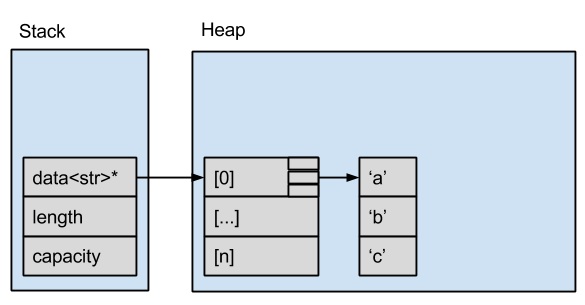
\includegraphics[scale=0.5]{figures/cpp_abstractions}
  \end{center}
  \caption{Abstractions of a Vector of Strings in Rust and C++.}
  \label{fig:cpp_abstractions}
\end{figure}

\subsection{Guaranteed memory safety}

One of Rust's biggest features is full memory safety \cite{web:rust_book_unsafe} without sacrificing performance.
The memory safety boils down to how Rust manages the variables and data-segments throughout the program.
Rust introduces a few concepts that are all centered around the \emph{ownership} of these variables, how the variables are \emph{borrowed} and the \emph{lifetimes} of the variables and the borrowed references to them.
Rust's ownership system are part of all the zero-cost abstractions mentioned in \autoref{chap:zero_cost_abstractions}, since all borrow-checking, and ownership- and lifetime-analysis are done statically at compile-time.

\subsubsection{Ownership and Move Semantics}
\label{sec:back:rust:own}

In order to achieve full memory safety, we have to remove all form for memory leaks and dangling pointers to invalid memory.
This implies one \emph{memory deallocation} for every respective \emph{memory allocation}.
Traditionally, when allocating memory for a variable, the programming language will return a \emph{pointer},  or a \emph{handle}, that is essentially an address to a record in memory, together with how many bytes it takes to store the record in memory.
When there is no longer any need for the memory it have to be deallocated.

Modern programming languages, like Java and Python, typically achieves this with a Garbage Collector that runs during program execution with the sole purpose of keeping the memory intact.
A common implementation is a reference counted garbage collector that keeps a count over the number of references to the variables and deallocates them when there are no valid references to them.
The downside of such an approach to memory safety is the continuous use of resources it requires to keep track all the references, every assignment and every time the variable enters a scope the reference count must be increased, and when it leaves a scope it must be decreased.

Another common implementation is a stop-the-world garbage collector.
It works differently, by regularly halting the executing program, and then tracing all references that are accessible from the root scope and the registers recursively.
The memory that are accessible from these references is then marked as valid, and all the invalid memory will then be freed and accessible through new calls to memory allocations.
The downside of such an approach is the requirement of halting the entire program in order to release the invalid memory.
There are also many other techniques of garbage collection, that are often a variation of the ones already described, but they are all troublesome in constraint environments such as found on a small embedded device, or in real-time systems where the unpredictability of program execution introduced by a garbage collector is unacceptable.

Another approach to keeping track of the memory resources have been to give the programmer full control of every memory allocation and deallocation.
This is the most common approach for systems programming languages like C and C++, where performance and predictability is important.
However, it is easier to make the mistakes of referencing invalid memory, or forgetting to free up memory that might lead the program to use all available resources over time.
This will inevitably lead the program to crash when it tries to allocate more memory when there are no memory left to allocate.

\todo{This subsection about GC and memory handling might be better suited in a different
background chapter}

It is important to always remember and deallocate all memory referenced by a handle, before the handle leaves its scope in the program.
Rust operates a little different from C when it comes to freeing memory, any variables holding a reference to stack- or heap-allocated memory will automatically be freed when it leaves the scope it lives in.
This is done statically without any interference of the programmer.
When the compiler sees that the handle for the allocated memory leaves its scope, it knows that it is lost to the program, so it will insert a call to free the memory at the moment it leaves the scope and becomes unreachable.
This eliminates the need for the programmer to manually do the memory bookkeeping.
These two aspects of memory allocation and deallocation is combined into the concept of \emph{ownership} that Rust incorporates.
When a handle that \emph{owns} a reference to a data-segment on the heap leaves its scope, Rust knows that it can safely free the memory that is referenced by it since it is the \emph{owning handle} of the memory, that can no longer be used in the program.
An example this ownership is shown in \autoref{lst:owning_handle}.

\begin{listing}[tb]
\begin{minted}{c}
struct Book { pages: u32 }

fn main() {
  // `b' is the owning handle to a Book
  let b = Book { pages: 150 };

  // when this line is reached, `read_book' takes ownership of `b'
  read_book(b);
  // when `read_book' returns, the book is also deallocated

  // this makes it impossible to  read the book two times
  read_book(b); // <- error: use of moved value: `b'
 }
\end{minted}
\caption{Owning handle}
\label{lst:owning_handle}
\end{listing}

There can only exist one owning handle for any heap- or a stack-allocated variable at any time during program execution.
This means that if the handle gets passed as an argument to a function, this function will take \emph{ownership} of the variable, by \emph{moving} it to the new scope defined by the function.
This move prevents any further use of the handle in its original scope and is necessary because Rust only allows one owned handle to any memory-segment at any time.
If two or more handles to the memory had existed at the same time it would have resulted in several calls to \emph{free}, one for every time the handle left the different scopes.
The only way to continue using the handle in its original scope would have been to give the ownership back after using it.

\subsubsection{Borrowing}

\emph{Borrowing} is introduced as an alternative to moving the variable ownership across multiple scopes.
Rust allows the programmer to \emph{lend} away access to handles by passing a reference to the variable around instead of the actual handle itself.
There can exist multiple \emph{references} to the same place in memory, as long there is only one \emph{owner} of the handle itself.
A reference is denoted with an \texttt{\&} in front of the handle, this will tell Rust that we're working with a reference to the handle, or just borrowing the handle to the end of the active scope.
Consider a modification of the previous example shown in \autoref{lst:borrowing_handle}.
Here, the the \texttt{read\_book} function is modified to accept references to book instead of taking ownership of it, this allows us to lend out the book to be read as many times as we want.

\begin{listing}[tb]
\begin{minted}{c}
fn main() {
  // `b' is the owning handle to a Book
  let b = Book { pages: 150 };

  // only a reference to the book is given to `read_book'
  read_book(&b);

  // it is possible to read the book two times, because `b'
  // still lives in the scope defined by the `main' function
  read_book(&b); z
 }
\end{minted}
\caption{Borrowing handle}
\label{lst:borrowing_handle}
\end{listing}

\subsubsection{Lifetimes}

Rust needs a way to ensure that the memory used by all borrowed references to a handle is intact, i.e. that the references does not point to any deallocated memory.
Rust achieves this with a concept called \emph{lifetimes}, in which the compiler with the help of \emph{lifetime elisions}, can statically resolve any dangling pointers or \emph{use-after-free} issues introduced by the programmer.
Consider the example shown in \autoref{lst:invalid_ref_c}, of a function in \texttt{C} that returns a reference into a variable allocated in its own stackframe.
The \texttt{C} compiler will issue a warning of such a serious mistake \todo{Error? Mistake? Fault?}, but it will still let you do it.
A similar implementation of \texttt{get\_ref} in \rust is shown in \autoref{lst:invalid_ref_rust}, but this will issue a compilation error because \texttt{n}'s lifetime is only valid for the scope defined by \texttt{get\_ref} itself, but not in the surrounding scope.

\begin{listing}[tb]
\begin{minted}{c}
int *get_ref() {
    int n = 3;
    return &n;
}
\end{minted}
\caption{Returning an invalid reference in C}
\label{lst:invalid_ref_c}
\end{listing}

\begin{listing}[tb]
\begin{minted}{rust}
fn get_ref() -> &i32 {
    let n = 3;
    &n // <- error: `n' does not live long enough
}
\end{minted}
\caption{Attempting to return an invalid reference in Rust}
\label{lst:invalid_ref_rust}
\end{listing}

Lifetime elisions are applied to structures and trait declarations, among others, and they are used in function definitions in order to tell Rust that the named lifetime is valid in the surrounding scope.
\todo{Sentence is unclear. Needs rewrite}
Such elisions are used extensively together with parameters and return values, and helps the compiler to reason about the liveliness of the references and whether they are valid or not.
There are two kinds of lifetimes; the ones associated with \emph{input parameters} to a function, and the ones associated with the \emph{returned value} from a function.
These are referred to as \emph{input-lifetimes} and \emph{output-lifetimes}, respectively.
We have an error if a function returns a value with an output lifetime that is not the same as the input lifetime, because this would have resulted in use-after-free.

Consider an updated version of the \texttt{get\_ref} function shown in \autoref{lst:invalid_ref_lifetimes_rust}, where the lifetime with the name \texttt{'a} is annotated by the function and tells the compiler that the value returned by the function has an output lifetime that lives longer than the function.
We do however still have a problem, it is clear from the code that \texttt{n} is allocated within the scope of \texttt{get\_ref}, and clearly does not have the input lifetime \texttt{'a}
As stated earlier, the only way we can return such a reference is if an input parameter has the same lifetime as the output-lifetime, a third, and working example of our problem is shown in \autoref{lst:valid_ref_rust}.

\todo{Bad explanation. Should probably switch out the example to e.g. returning a reference to the number of pages in a book?}

\begin{listing}[tb]
\begin{minted}{rust}
fn get_ref<'a>() -> &'a i32 {
    let n = 3;
    &n
}
\end{minted}
\caption{Attempting to return a reference with lifetime elisions}
\label{lst:invalid_ref_lifetimes_rust}
\end{listing}

\begin{listing}[tb]
\begin{minted}{rust}
fn get_ref<'a>(n: &'a i32) -> &'a i32 {
    &n
}
\end{minted}
\caption{Retuning a reference with correct use of lifetime elisions}
\label{lst:valid_ref_rust}
\end{listing}

\todo[inline]{I have mixed the use of data-segments, variables, pointers and handles. They should be properly defined and used within the right contexts.}

\subsection{Big-Stack allocation}
\label{par:big_stack}

Rust uses "big stack" allocations and does a good job of avoiding dynamic heap allocation of data.
\todocite{need big-stack citation. I think I've read about it somewhere}
Combined with Rust's strong lifetime semantics, it is possible to write larger programs that are fully stack-allocated, with little or no dynamic heap allocations.
This can significantly boost performance as the need for garbage collectors and other runtime requirements is minimal (important for embedded devices).

\todo{Just rambling along to get an idea of something to write.}

% subsubsection memory_safety (end)

\subsection{Concurrency Model} % (fold)
\label{ssub:concurrency_model}

Rust has a concurrency model. Duh.
\todo {We should mention this shortly. This is not something that is very relevant for our project, but it is relevant for rust itself.}

% subsubsection concurrency_model (end)

\subsection{Unsafe Code} % (fold)
\label{ssub:unsafe_code}

The strong type system along with lifetime inference and borrow-checking help Rust become a safe language.
The language provides safe, zero-cost abstractions over the machine it is running on, but it is not always possible to guarantee full safety without sacrificing performance, or vice versa.
Achieving good performance is often a synonym with direct memory access and pointer manipulation, which in itself is not considered to be safe operations.
\todo{At least by Rust. Depends on who considers it.}

% subsubsection unsafe_code (end)

\subsection{Organization}
\label{ssub:rust:organization}

\subsubsection{Crates and Modules}

Rust provides two main features to organizing code, crates and modules.
A crate defines a collection of modules which constitutes a library.
The crate construct is a sharable part of rust code that can be included into other projects and libraries.
The module is the hierarchical means of organizing a crate.
Figure \ref{fig:rust:collections} shows a few or the modules contained within the Rust collection library.

\begin{figure}[H]
  \begin{center}
    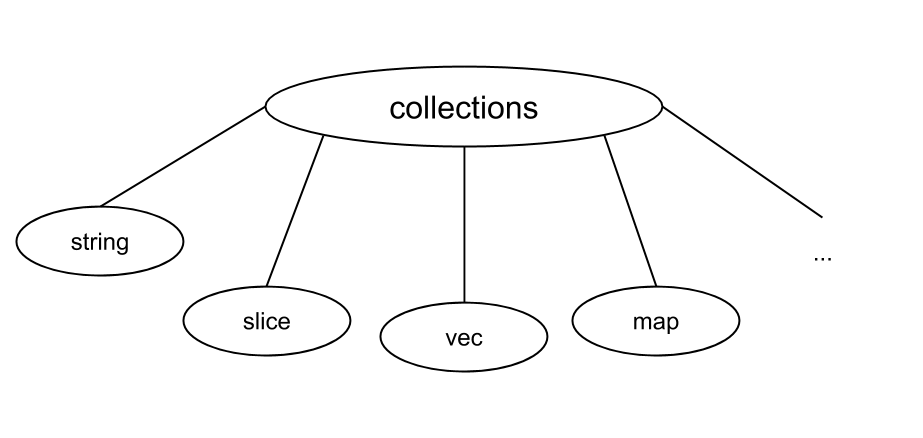
\includegraphics[scale=0.3]{figures/background/rust/libcollections.png}
  \end{center}
  \caption{Modules in collection crate.}
  \label{fig:rust:collections}
\end{figure}

\subsubsection{Rust library}

The Rust library is organized using crates.
This ensures that the design is modular and provides the programmer the ability to import only the components of the library that is needed for a given program.
The \texttt{Cargo} packages manager makes this feature easily exploitable.
Usually this facility is not needed when writing Rust programs, but when targeting embedded platforms barebones \todo{Bare metal?} this is integral to exploiting the standard library.
As the standard library contains functionality that assumes a operating system the library as a whole cannot be utilized.
Figure \ref{fig:rust:librust} depicts the crates of the standard library with their dependencies.

\begin{figure}[H]
  \begin{center}
    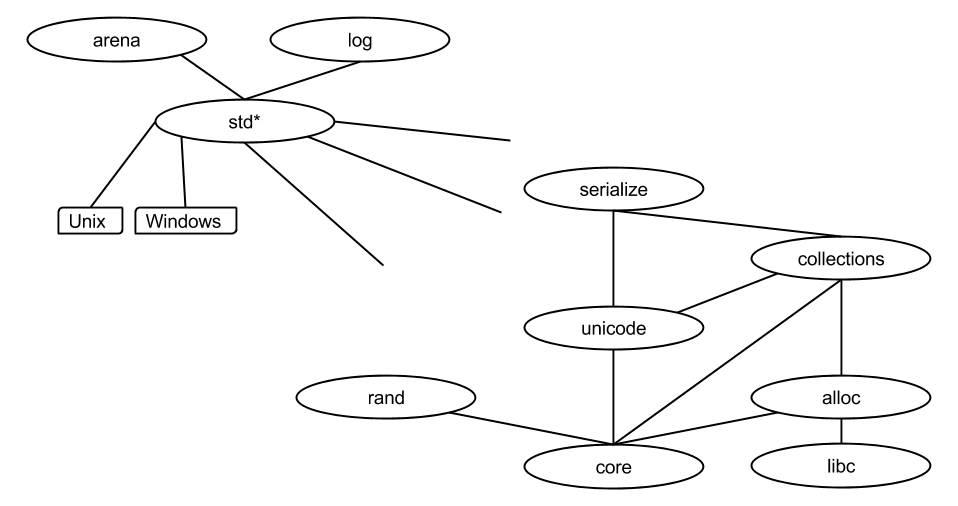
\includegraphics[scale=0.3]{figures/background/rust/rust-lib.png}
  \end{center}
  \caption{Some crates of the rust library}
  \label{fig:rust:librust}
\end{figure}
std* - The std crate depends nearly all of the crates in the lower right corner

\subsection{Cargo}
\label{sec:cargo}

\texttt{Cargo} is Rust's package manager, a program that automates the process of building Rust programs.
It comes bundled with the default installation of Rust.
\texttt{Cargo} comes with a collection of tools that makes building, testing and running Rust programs a lot easier than invoking \texttt{rustc} directly.
\texttt{Cargo} also defines a standard Rust project layout, in addition to downloading and updating package dependencies.
This section will cover the most important features of \texttt{Cargo} and how it works that is required in order to understand the work that is described later in this project report.

\subsubsection{Project Structure}

Every crate, or package, built by \texttt{Cargo} requires a \texttt{Cargo.toml} file to be present in the root directory.
This file is interpreted by \texttt{Cargo} and is used to determine the name of library and executables to be built in the package and what other packages that it depends on.
It also includes information that tells \texttt{Cargo} how the package can be compiled for different target architectures, and it is used to define different \textit{features} of a package - a way to conditionally compile certain parts of the code present in the library.

\begin{listing}
\dirtree{%
.1 hello\_world.
.2 Cargo.lock.
.2 Cargo.toml.
.2 build.rs
.2 src.
.3 bin.
.4 hello\_mars.rs.
.4 hello\_jupiter.rs.
.3 lib.rs.
.3 main.rs.
.2 examples.
.3 hello\_venus.rs.
.2 tests.
.3 hello\_planets\_test.rs.
}
\caption{Cargo project structure}
\label{lst:cargo_project_structure}
\end{listing}

\autoref{lst:cargo_project_structure} shows a standard \texttt{Cargo} project structure.
The \texttt{lib.rs} file will be compiled into a crate with the project name, in this case it will be \texttt{hello\_world.rlib}.
If a \texttt{main.rs} file is present, it will be compiled into an executable with the same name.
Any files found under the \texttt{src/bin} directory will also be compiled into its own executables, \texttt{Cargo} will automatically link the \texttt{hello\_world} library and all of the package dependencies with these executables.
The \texttt{examples} directory contains different executables that demonstrates how to use the library, and finally the \texttt{tests} directory contains integration tests.
A package can also have it's own build-routine by specifying a \texttt{build} file in \texttt{Cargo.toml}, in this case we have a \texttt{build.rs} file present in the project.
This file is executed prior to building the library itself, and provides the possibility to e.g. compile and link third party C-libraries, or e.g. generated code prior to compilation.
Finally, \texttt{Cargo} also generates a \texttt{Cargo.lock} file that contains information about every package that are used by the project library and executables.
This file helps \texttt{Cargo} to determine if packages needs to be re-downloaded, updated or re-compiled in order for the package to behave correctly and be built consistently - independent on the target architecture it is built on, and for.

\subsubsection{Building and testing (Or Tools?)}

As mentioned earlier, \texttt{Cargo} comes with a collection of tools that makes it easy to build and test Rust projects.
The most common commands are shown in \autoref{tab:common_cargo_commands}.
Most of these tools are self explanatory, but the \texttt{build} and the \texttt{test} commands will be described a little more thoroughly in this section.

\begin{table}[ht]
\begin{center}
\begin{tabular}{r|l}
\textbf{Command} & \textbf{Description}                           \\
\hline
build  & Compile the current project                              \\
clean  & Remove the target directory                              \\
doc    & Build this project's and its dependencies' documentation \\
new    & Create a new cargo project                               \\
run    & Build and execute src/main.rs                            \\
test   & Run the tests                                            \\
bench  & Run the benchmarks                                       \\
update & Update dependencies listed in Cargo.lock                 \\
\hline
\end{tabular}
\caption{Common cargo commands}
\label{tab:common_cargo_commands}
\end{center}
\end{table}

By invoking the \texttt{cargo build} command, \texttt{Cargo} will download and resolve all package dependencies, and trigger \texttt{rustc} to compile them and link them with each other in the correct order.
When all dependencies have been built, the build script will be invoked (if it is present in the package), before the library itself is compiled.
Lastly, if the project contains a \texttt{main.rs} or sources in the \texttt{src/bin} directory, the projects executables will be compiled.

The \texttt{cargo test} command will also trigger \texttt{rustc} to compile the library in the same manner as \texttt{cargo build}, but it will leave out compilation of the project executables.
When the library is compiled, any function that is marked with \texttt{\#[test]} will be included and treated like a unit test, this is a feature from Rust itself.
\texttt{Cargo} also treats all the sources found in the \texttt{examples} directory as tests, so these will be compiled instead of the other project executables, together with all the integration tests.
When \texttt{Cargo} has finished compiling the library and its executables, it will by default run all the unit tests, including the integration tests, but it will not run the examples.

\begin{table}[ht]
\begin{center}
\begin{tabular}{r|l}
\textbf{Flag} & \textbf{Description}                                   \\
\hline
--features FEATURES   & Space-separated list of features to also build \\
--target TRIPLE       & Build for the target triple                    \\
\hline
\end{tabular}
\caption{Cargo flags to alter the package library and executables}
\label{tab:cargo_flags}
\end{center}
\end{table}

Both of these commands support several optional build-specific flags that are passed further on to the invocation of \texttt{rustc}, we will take extra notice to the two flags shown in \autoref{tab:cargo_flags}.
The \texttt{--target} flag is used if the project should be compiled for a different target architecture than the machine it is invoked on, this is necessary when cross-compiling the package.
The list following the \texttt{--features} flag will be used by \texttt{Cargo} and \texttt{rustc} to conditionally compile code that is present in the project.
Consider the example shown in \autoref{lst:rust_features} and its output shown in \autoref{tab:rust_features_output}.
We can see from this example that the definition of the \texttt{num} function will be different based on the feature flag that is passed together with \texttt{Cargo}.

\begin{listing}[H]
\begin{minted}{rust}
// src/main.rs
#[cfg(feature = "one")]
fn num() -> u32 { 1 }

#[cfg(feature = "two")]
fn num() -> u32 { 2 }

fn main() {
    println!("num() + num() = {}", num() + num())
}
\end{minted}
\caption{Example usage of features}
\label{lst:rust_features}
\end{listing}

\begin{table}[ht]
\begin{center}
\begin{tabular}{r|l}
\textbf{Command} & \textbf{Output}                          \\
\hline
\texttt{\$ cargo build --features one}  & num() + num() = 2 \\
\texttt{\$ cargo build --features two}  & num() + num() = 4 \\
\hline
\end{tabular}
\caption{Example output of features}
\label{tab:rust_features_output}
\end{center}
\end{table}
